\chapter{\ifproject%
      \ifenglish Project Structure and Methodology\else โครงสร้างและขั้นตอนการทำงาน\fi
  \else%
      \ifenglish Project Structure\else โครงสร้างของโครงงาน\fi
  \fi
 }



\makeatletter

% \renewcommand\section{\@startsection {section}{1}{\z@}%
%                                    {13.5ex \@plus -1ex \@minus -.2ex}%
%                                    {2.3ex \@plus.2ex}%
%                                    {\normalfont\large\bfseries}}

\makeatother
%\vspace{2ex}
% \titleformat{\section}{\normalfont\bfseries}{\thesection}{1em}{}
% \titlespacing*{\section}{0pt}{10ex}{0pt}

\section{\ifenglish Story line\else ภาพรวมของเกม\fi }
เป็นเกมที่จะมีเรื่องราวให้ผู้เล่นได้สวมบทบาทและเผชิญหน้ากับสิ่งที่น่าหวาดกลัว ความกดดัน และเอาตัวรอดจากสถานการณ์ต่าง ๆ ในเกม ซึ่งเป็นแนวเกมที่ได้รับความนิยมในยุคปัจจุบัน โดยในโครงงานนี้ จะเป็นการพัฒนาเกมแนวสยองขวัญ ที่มีมุมมองบุคคลที่ 3 แบบด้านข้าง โดยผู้เล่นจะได้รับบทบาทเป็นนักเรียนคนหนึ่ง ที่มีเพื่อนสนิทพยายามฆ่าตัวตาย แต่ไม่สำเร็จ และนอนไม่ได้สติอยู่ในโรงพยาบาล ผู้เล่นจะต้องค้นหาความจริง โดยการไขปริศนาต่าง ๆ และต้องเอาตัวรอดจากอุปสรรคที่คอยรบกวนผู้เล่น ไม่ให้ไปถึงความจริง และต้องการจะปลิดชีพผู้เล่น ระบบของเกมจะถูกออกแบบให้ผู้เล่นจะต้องคอยบริหารค่าพลังงานที่ใช้ในการทำกิจกรรมต่างๆ ค่าสติที่มีผลกับการรับรู้ของตัวละคร และเวลาที่มีอยู่อย่างจำกัด ซึ่งข้อจำกัดเหล่านี้จะส่งผลให้ผู้เล่นมีความกดดันในการตัดสินใจเลือกการกระทำ สำหรับการดำเนินเนื้อเรื่องและฉากจบ จะมีการเปลี่ยนแปลงไปตามการเลือก ข้อมูล และไอเทมที่ได้รับในระหว่างเล่นเกม


% \section{\ifenglish Work flow game\else ลำดับการทำงาน\fi}
% \begin{figure}[h]
%     \centering
%     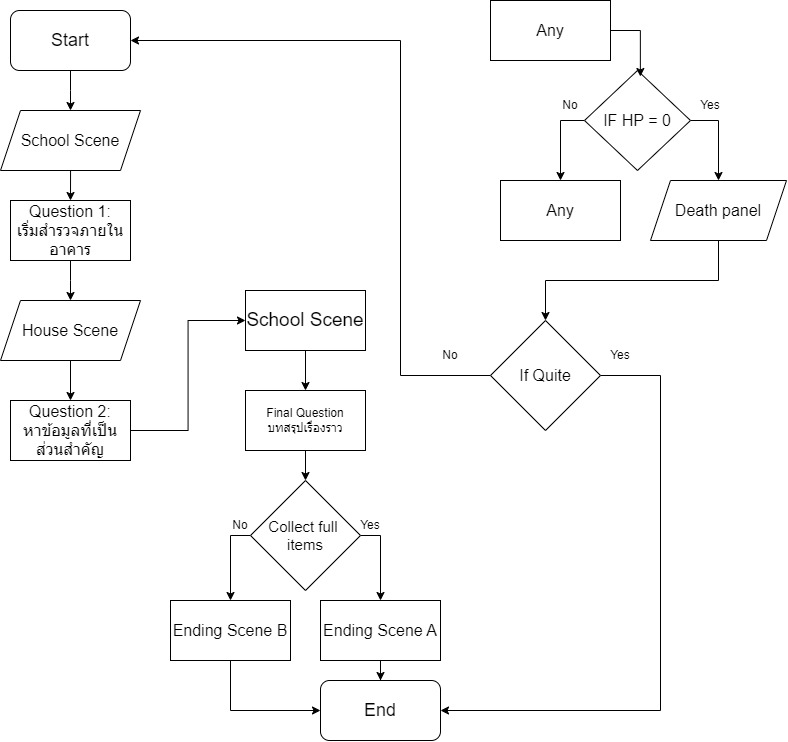
\includegraphics[width=\textwidth, height=0.5\textheight]{Images/FlowChart.jpg}
% \end{figure}

\section{\ifenglish Story board\else เนื้อเรื่องภายในเกม\fi}

\textbf{intro}
เช้าวันหนึ่งที่ไปโรงเรียน มีดอกไม้และข้อความแปลก ๆ วางอยู่บนโต๊ะของเพื่อนสนิท ยังไม่ทันได้หายสงสัย ครู
ประจําชั้นก็เข้ามาในคาบ homeroom และได้พูดขึ้นว่า เพื่อนของเขาหรือแพรวนอนไม่ได้สติอยู่ที่โรงพยาบาล อาการ
สาหัสมาก แต่ไม่ทราบสาเหตุ ทําให้เขานั้นไม่เชื่อและเกิดความคิดที่อยากจะหาความจริงเกี่ยวกับเรื่องนี้ เลยมุ่งหน้าไปที่โรงพยาบาล และแอบเข้าไปดูแพรวในห้องพักผู้ป่วยฉุกเฉิน โดยการหลอกกดปุ่มสัญญาณเตือนไฟไหม้ ทำให้พยาบาลต่างก็วิ่งหนีออกมา ในขณะนั้นเขาจึงเข้าไปที่เคาท์เตอร์พยาบาลเพื่อทำการค้นหาชื่อแพรวและเลขเตียง จากนั้นเขาจึงออกตามหาตามห้องที่ได้บอกไว้ จึงได้พบว่าสิ่งที่ครูประจําชั้นพูดนั้นเป็นความจริง หลังจากนั้นเราก็ได้เดินออกมาจากห้องพักผู้ป่วยด้วยความรู้สึกสงสัยปนเศร้า ทันใดนั้นก็มีแสงวาบเกิดขึ้น และตัวเขาก็ได้ย้อนไปในอดีตเพื่อรับรู้และแก้ไขเรื่องราวได้สมใจ โดยเรื่องราวหลังจากย้อนไปในอดีตนั้น จะย้อนเวลาไป 1 วันก่อนที่แพรวจะลงมือฆ่าตัวตาย โดยเริ่มจากที่บ้าน
 
\textbf{chapter1}
ซึ่งเหตุการณ์ภายในบ้านนั้นจะมีฉากการทะเลาะกับของแพรวกับแม่ และ มีการทำร้ายร่างกาย ด่าทอกันเกิดขึ้น เพราะแม่ไม่พอใจที่เพื่อนมีผลการเรียนที่ไม่ดี ถึงแม้วิชานั้นแพรวจะพยายามถึงที่สุดแล้วก็ตาม
พอทะเลาะกันเสร็จแม่จะเดินออกจากห้องของแพรว และเราก็เดินเข้าไปหาแพรวเพื่อปลอบโยน แต่พูดไปเท่าไรก็เหมือนจะไม่ได้ยินเพราะเธอกำลังร้องไห้อยู่ เลยทำได้แค่กอดเพื่อนไว้ หลังจากนั้นเราสามารถสำรวจห้องนอนของแพรวได้โดยการเดินไปรอบๆห้อง และเก็บของที่พอจะดูเป็นสาเหตุที่ทำให้แพรวเป็นแบบนั้น เช่นใบเกรดที่ถูกฉีกเนื่องจากการทะเลาะกับแม่เมื่อสักครู่ และเมื่อเราเดินออกจากห้องนอนของแพรวเพื่อจะกลับบ้าน กลับพบว่ามีวิญญาณร้ายกำลังเดินตามมาทำร้าย ทำให้ต้องหลบซ่อนโดยแอบในห้องน้ำ และพยายามทำทุกวิถีทางไม่ให้วิญญาณร้ายเปิดประตูได้ และหลังจากนั้นเราจะได้เบาะแสเพิ่มเติมจากวิญญาณ ก่อนที่จะหายไป 

\textbf{chapter2}
ต่อมาจะเป็นฉากในโรงเรียน ซึ่งแพรวก็ยังมาโรงเรียนตามปกติ ในสภาพยิ้มแย้มแจ่มใสเหมือนที่เคยเป็น แต่แล้วตอนคาบพักของวิชาหนึ่ง ได้มีเพื่อนที่ไม่ค่อยถูกกับแพรว มาแฉข่าวลือเรื่องคลิปหลุดระหว่างแพรวกับแฟนเก่าที่เพิ่งเลิกกันไปซึ่งเป็นแฟนปัจจุบันของเพื่อนคนนั้น แต่จริง ๆ แล้วในคลิปนั้นเป็นแค่คนหน้าเหมือนกันเท่านั้น แต่ทุกคนในห้องก็ตราหน้าเธอไปแล้วว่าเป็นนักเรียนที่ไม่ดี อีกทั้งแฟนเก่าของเธอก็ยังเพิกเฉยต่อข่าวข่าวนี้ ซึ่งในขณะนั้นเราก็สังเกตเห็นได้ว่า ตัวเราเองในอดีตนั้น ไม่ได้ออกมาปกป้องเพื่อนเลยแม้แต่น้อยเพราะกลัวว่าจะโดนลูกหลงไปด้วย เราเลยเริ่มเอะใจแล้วว่า หรือจริง ๆ แล้ว นี่ไม่ใช่การแก้ไขอดีต แต่เป็นการย้อนเวลามาดูอดีตต่างหาก อย่างไรก็ตาม หลังจากที่แพรวโดนตราหน้าไปแบบนั้น เธอจึงวิ่งหนีออกไปที่ห้องน้ำ เราจึงตามไปดูว่าแพรวไปที่ไหน ระหว่างที่เธอกำลังตามไปดู จู่ ๆ เราก็มีอาการคล้าย ๆ กับหน้ามืด และวิญญาณตัวนั้นก็โผล่มาอีกครั้ง ทำให้เราต้องวิ่งหนีเข้าห้องน้ำ และป้องกันไม่ให้วิญญาณร้ายเปิดประตูได้ แต่ครั้งนี้กลับไม่สำเร็จจึงโดนทำร้าย และก่อนที่วิญญาณจะจากไปมันได้บอกว่า"วันนี้ หัวค่ำ ดาดฟ้า" ซึ่งอาจจะเป็นเบาะแสอะไรบางอย่าง หลังจากวิญญาณหายไป เราก็ตามหาแพรวจากเสียงสะอื้นในห้องน้ำอีกครั้ง และพยายามเคาะประตู แต่ก็ไม่เป็นผล เพราะเหมือนเธอไม่ได้ยินอะไรเลย ทำให้เราต้องเดินออกมา ระหว่างที่เดินกลับไปที่ห้องเรียน เราก็ได้ยินผู้คนพูดถึงเรื่องคลิปหลุดของแพรว ทำให้เธอรู้ว่าข่าวลือนั้นได้สะพัดไปทั่วโรงเรียนแล้ว
เย็นวันนั้น แพรวไม่ยอมกลับบ้าน เพราะเธอกลัวว่าจะโดนแม่ของเธอต่อว่าอีก และเธอต้องการจะเคลียร์กับแฟนเก่าว่าทำไมถึงเกิดเรื่องแบบนี้ขึ้นกับเธอ แต่เธอก็โดนเขาต่อว่าอีกว่าเป็นคนไม่สวย เรียนก็ไม่เก่ง ใครจะอยากได้เป็นแฟน และที่ยอมคบกับอีกคนเพราะว่าจริง ๆ เขาได้แอบชอบผู้หญิงคนนั้นมานานแล้ว แต่เธอไม่ยอมรับรักสักที และรู้มาว่าเธอไม่ชอบแพรว เลยมาขอเป็นแฟนเพื่อให้เกิดความหึงหวงขึ้นและรับรักเขาในที่สุด ซึ่งมันก็ได้ผล ทำให้แพรวเสียใจมาก ถึงมากที่สุด และที่โดนปล่อยคลิปหลุดเพราะว่าเธอต้องการให้ทุกคนมองว่าแพรวเป็นคนไม่ดี และให้ทุกคนแบนเธอทิ้งไปซะ โทษฐานแย่งแฟนคนอื่น

\textbf{chapter3}
ด้วยความเสียใจแพรวจึงนั่งร้องไห้อยู่คนเดียวสักพักซึ่งมีเรานั่งอยู่ข้าง ๆ สักพักภาพก็มืดดำไป และตัดกลับมาที่เรายังนั่งอยู่ที่เดิม แต่แพรวไม่อยู่แล้ว ซึ่งจะเดินออกจากโรงเรียนก็ไม่ได้ เพราะเป็นเวลาที่ประตูโรงเรียนปิดแล้ว ทำให้เรานึกคำใบที่วิญญาณพูดกับเธอได้ว่า"วันนี้ หัวค่ำ ดาดฟ้า" เราจึงวิ่งเข้าไปในอาคารเรียน แต่อาคารเรียนล็อก ทำให้ต้องไปหากุญแจมาเปิดให้ได้ ซึ่งก็หาเจอแต่นั่นก็ทำให้วิญญาณร้ายปรากฏตัวอีกครั้ง แต่เวลาเหลือไม่มากแล้ว เลยต้องวิ่งขึ้นไปบนดาดฟ้าให้ทันเพื่อไปดูว่าจะเกิดอะไรขึ้นกับแพรว โดยที่ยังมีวิญญาณวิ่งตามหลัง พอขึ้นไปถึงด้านบน เราจึงตะโกนเรียกชื่อเพื่อนของเธอ ทำให้แพรวที่กำลังจะกระโดดลงจากตึกนั้นชะงักและหันมามอง เราจึงเข้าไปจับมือและห้ามไม่ให้เพื่อนกระโดด แต่เธอก็ยังยืนยันที่จะจบชีวิตตัวเอง เธอเกลียดตัวเอง เกลียดมากซะจนอยากจะฆ่ามันทิ้งไปซะ ไม่มีใครรักเธอแล้ว เธอล้มเหลวทุกอย่างในชีวิต ทันใดนั้นวิญญาณร้ายก็ได้โผล่ขึ้นมา ซึ่งเราหมดหนทางหนีแล้ว ทำให้ต้องต่อสู้และระหว่างการต่อสู้นั้นทำให้แพรวเห็นว่า ยังมีคนที่อยู่เคียงข้างมาตลอด แค่ระหว่างทางนั้นเราไม่กล้าที่จะพูดหรือแสดงออกเพราะกลัวสังคมตราหน้า แต่ตอนนี้เธอไม่กลัวอะไรอีกแล้ว ระหว่างที่สู้กับวิญญาณร้ายเราพลาดท่าและตกตึกลงไปแทนแพรว แพรวที่เห็นดังนั้นก็เป็นลมสลบไป และยามที่เห็นว่ามีคนร่วงมาจากดาดฟ้าและเห็นว่ามีคนยืนอยู่ก็ได้ขึ้นมาช่วยแพรวไว้ และแจ้งตำรวจว่ามีนักเรียนตกตึกจึงนำตัวส่งโรงพยาบาลและเสียชีวิตในเวลาต่อมา

\textbf{last chapter}
2สัปดาห์ต่อมา แพรวได้รับความยุติธรรมว่าในคลิปนั้นไม่ใช่เธอ และทางโรงเรียนก็เอาผิดเพื่อนคนนั้นที่ปล่อยข่าวลือโดยการพักการเรียน 1 เทอมการศึกษา ทำให้แพรวได้กลับมาใช้ชีวิตในรั้วโรงเรียนได้อีกครั้ง แต่เธอก็ยังยืนยันว่าจะลาออกจากโรงเรียนที่นี่แล้วย้ายบ้านออกไปอยู่กับพ่อ เนื่องจากเธอได้แจ้งตำรวจไปเมื่อวันที่เธอจะทำการฆ่าตัวตาย ว่าแม่ของเธอมีการใช้กำลังเกิดขึ้น ทำให้เรื่องไปถึงพ่อ พ่อจึงฟ้องหย่ากับภรรยา และขอสิทธิ์เลี้ยงดูลูกทำให้เธอต้องย้ายไปต่างจังหวัดเพื่ออยู่กับพ่อ อย่างไรก็ตามเธอมาโรงเรียนวันสุดท้ายเพื่อเก็บของ และเห็นว่ามีดอกไม้วางอยู่บนโต๊ะ พร้อมข้อความให้กำลังใจเธอเต็มไปหมด เช่น ขอให้เธอปลอดภัย แต่ถัดไปโต๊ะอีกตัว ซึ่งเป็นโต๊ะของเรา ไม่มีแม้แต่เศษกระดาษมาวางไว้ ทั้ง ๆ ที่เราได้ตายไปแล้ว แพรวจึงวางดอกไม้สีขาวไว้บนโต๊ะเรา เพื่อเป็นการไว้อาลัย ก่อนที่เธอจะเดินออกจากห้องไปเพื่อเริ่มต้นชีวิตใหม่


\section{\ifenglish Story line\else องค์ประกอบภายในเกม\fi }
\subsection{\ifenglish Story line\else ตัวละคร\fi }
ในที่นี้ จะแบ่งเป็นตัวละครหลักและตัวละคร
\subitem ตัวละครหลัก
\begin{itemize}
    \item \textbf{ตัวเอก} เป็นนักเรียนหญิงชั้นมัธยมปลาย ผมสั้น สวมใส่แว่น มีลักษณะนิสัย เป็นคนเงียบๆ มีเพื่อนน้อย ไม่ค่อยมีมนุษย์ปฏิสัมพันธ์
    \begin{figure}[h]
        \centering
        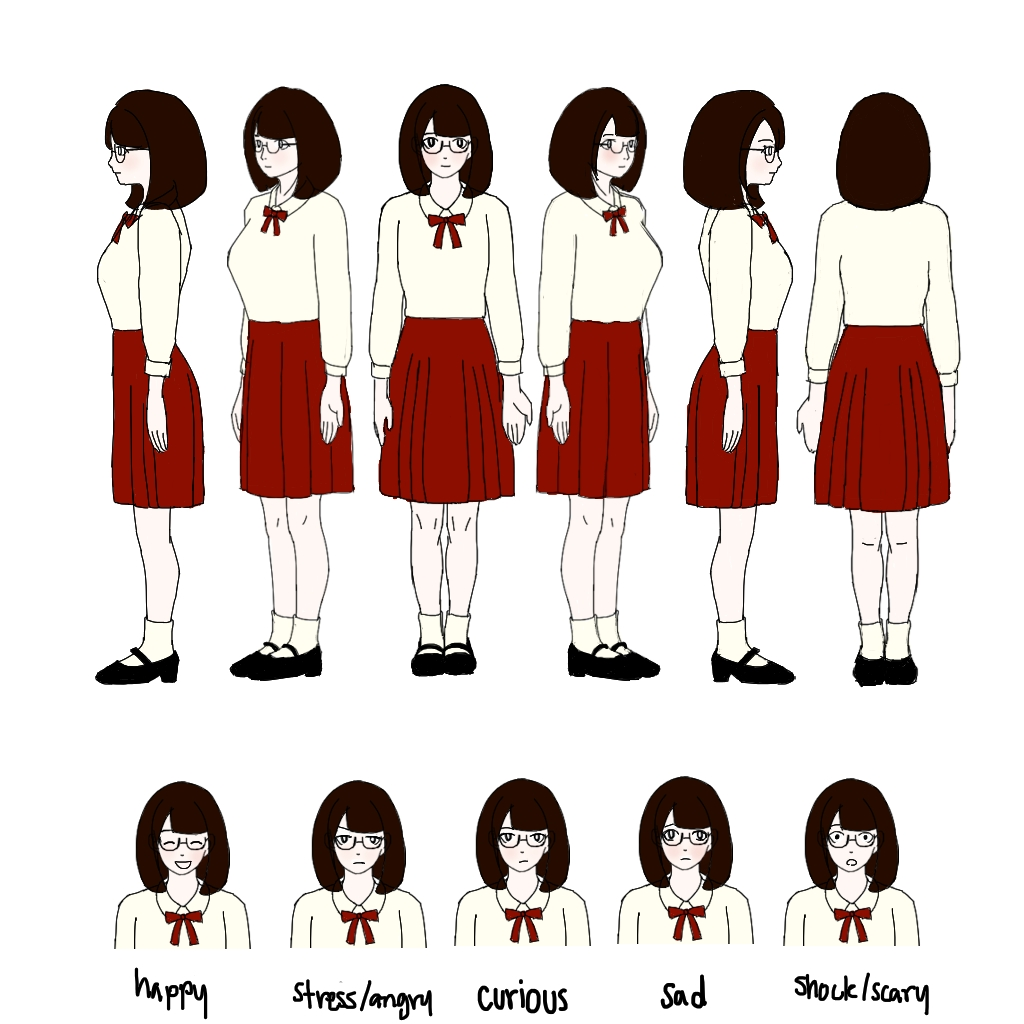
\includegraphics[width=0.6\textwidth, height=0.3\textheight]{Images/demo_character.jpg}
        \caption{ภาพ sketch ตัวละครหลัก}\label{MainCharacter}
    \end{figure}
    \item \textbf{แพรว} เป็นนักเรียนหญิงชั้นมัธยมปลาย ผมยาว มีลักษณะนิสัย เป็นคนจริงจังกับทุกๆเรื่อง และต้องการทำทุกๆอย่างให้สมบูรณ์แบบมากที่สุด เพื่อเอาใจคนรอบข้าง
    \begin{figure}[h]
        \centering
        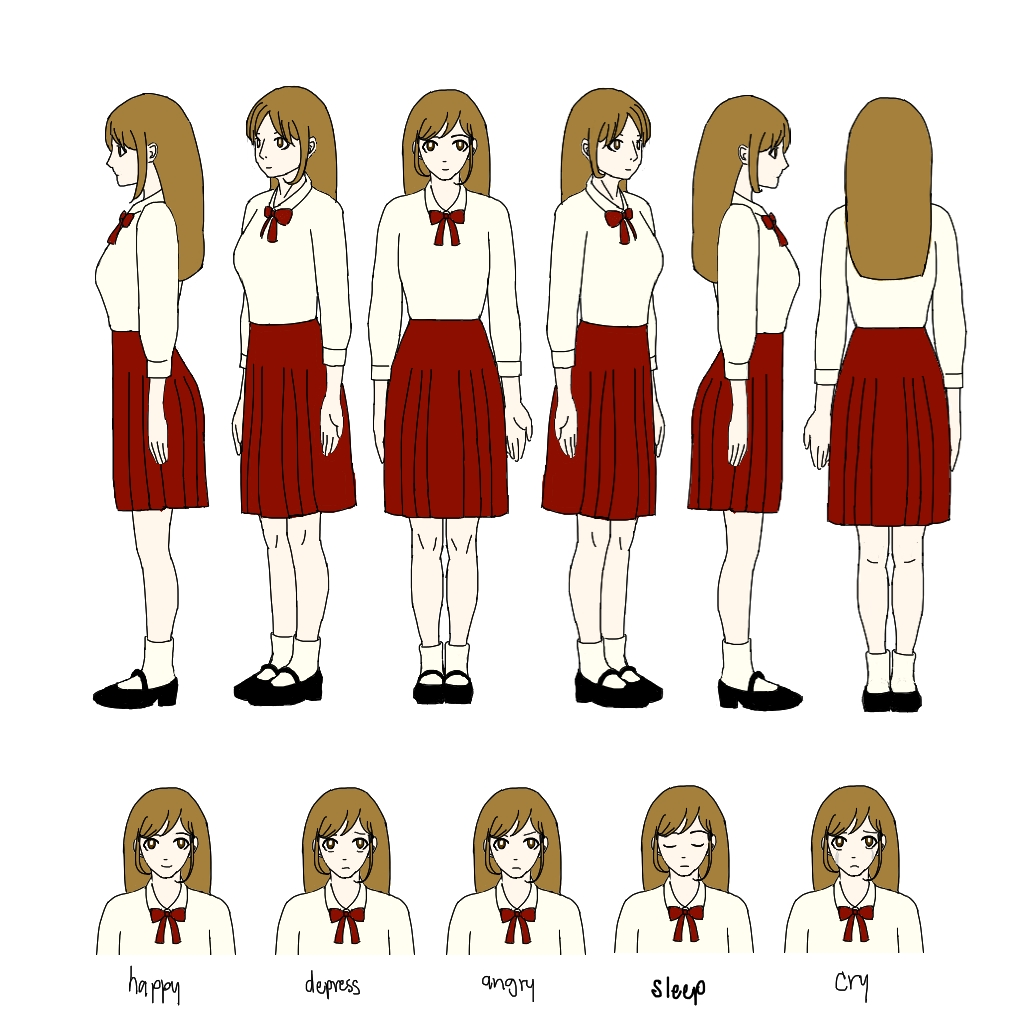
\includegraphics[width=0.6\textwidth, height=0.3\textheight]{Images/demogame_character.jpg}
        \caption{ภาพ sketch แพรว}\label{PrawCharacter}
    \end{figure}
    \item \textbf{วิญญาณร้าย} ผู้หญิงผมยาวสีดำ ดวงตามีสีดำล้วนเหมือนจะกลวงโบ๋ มีคราบน้ำตาสีเลือดเปื้อนอยู่ที่แก้ม มีลักษณะนิสัย ทุก ๆ ครั้งที่เราจะรู้ความลับของแพรว มันจะปรากฎตัวและทำร้ายเรา ซึ่งเป็นนิสัยอีกด้านของแพรว ที่ไม่ต้องการให้ใครมารับรู้ความลับที่เธอเป็นคนไม่สมบูรณ์แบบ
    \begin{figure}[h]
        \centering
        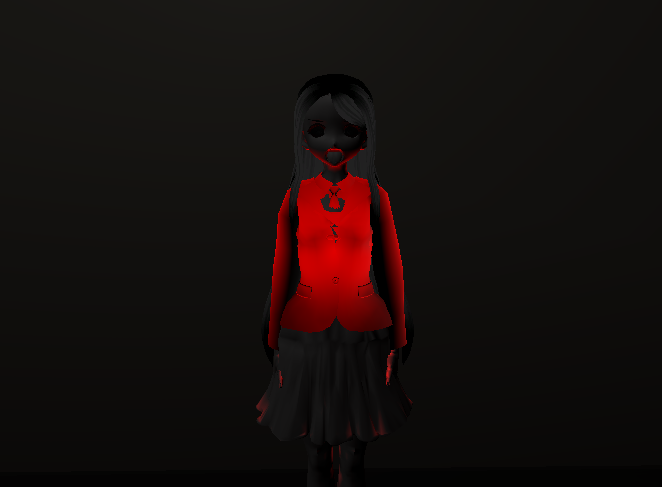
\includegraphics[width=0.6\textwidth, height=0.3\textheight]{Images/enemylv.1_character.jpg}
        \caption{ภาพ sketch วิญญาณร้าย}\label{GhostCharacter}
    \end{figure}
\end{itemize}

\subitem ตัวละครเสริม
\begin{itemize}
    \item \textbf{ครูประจำชั้น} เป็นผู้หญิงวัยผู้ใหญ่  ผมยาวประบ่า สวมชุดสุภาพ
    \item \textbf{พยาบาล} เป็นผู้หญิงวัยผู้ใหญ่ เก็บผมเรียบร้อย สวมเครื่องแบบพยาบาล
    \item \textbf{รปภ.} เป็นผู้ชายวัยกลางคน ผมสั้น สวมเครื่องแบบรปภ.
    \item \textbf{นักเรียนหญิง} เป็นผู้หญิงผมยาวประบ่าสีดำ สวมเครื่องแบบนักเรียน
    \item \textbf{นักเรียนชาย} เป็นผู้ชายผมสั้น  สวมเครื่องแบบนักเรียน
    \item \textbf{แม่} เป็นผู้หญิงวัยกลางคน ผมสั้น สวมชุดอยู่บ้าน
\end{itemize}

\subsection{\ifenglish Story line\else ฉาก\fi }
\begin{itemize}
    \item \textbf{โรงเรียน} เป็นอาคาร 3 ชั้น แต่ละชั้นมีห้องเรียน 6 ห้อง มีทั้งห้องเรียน ห้องน้ำ และทางเดินหน้าโรงเรียน
    \item \textbf{โรงพยาบาล} เป็นอาคาร 8 ชั้น ประกอบไปด้วย เคาท์เตอร์พยาบาล และห้องฉุกเฉิน
    \item \textbf{บ้าน} เป็นอาคาร 2 ชั้น ประกอบไปด้วยห้องนอนแพรว
\end{itemize}

\subsection{\ifenglish Story line\else การควบคุมตัวละคร\fi }
\begin{center}
    \begin{tabular}{|c|c|}
    \hline
    กดปุ่ม A, D & ใช้ในการเคลื่อนที่ของตัวละครให้เคลื่อนที่ไปทางซ้าย ทางขวา ตามลำดับ\\
    กดปุ่ม W, S ที่บันได& ใช้ในการขึ้นไปข้างบน หรือ ลงข้างล่าง\\
    กดปุ่ม E ที่วัตถุเช่น ประตูหรือกล่อง& ใช้ในการทำการ interaction เปิดประตูหรือเก็บของ\\
    กดปุ่ม E ที่ตู้ล็อคเกอร์หรือห้องน้ำ& เพื่อทำการซ่อนตัวจากศัตรู\\
    ขณะซ่อนตัว กดปุ่ม E& เพื่อยกเลิกการซ่อนตัว\\
    กดปุ่ม E ค้างที่ กล่องหรือโต๊ะเรียน & ใช้ในการเก็บ/ค้นหา items จากกล่องหรือโต๊ะเรียน\\
    กดปุ่ม I & ใช้ในการเปิด inventory ขึ้นมา\\
    กดปุ่ม Esc& ใช้ในการ puase game\\
    หน้า puase game กดปุ่ม Q& เพื่อออกจากการ puase game\\
    หน้า inventory กดที่ item& เพื่อเปิดดูข้อมูลของ items นั้นๆ\\
    หน้า inventory กดปุ่ม use& เพื่อทำการใช้ items นั้นๆ\\
    หน้า inventory กดปุ่ม drop& เพื่อทิ้ง items ที่ไม่ต้องการใช้งาน\\
    หน้า inventory กดปุ่ม กากบาท หรือ ปุ่ม Q& เพื่อปิดหน้า inventory\\
    กดปุ่มลูกศร& เพื่อใช้ในการกด Quick Time Event ที่จะมาในแบบลูกศร\\
    \hline
    \end{tabular}
\end{center}
\subsection{\ifenglish Story line\else ค่าพลัง\fi }
\begin{itemize}
    \item \textbf{ค่าพลังชีวิต} เป็นค่าที่จะส่งผลต่อการมีชีวิตของตัวละคร เป็นค่าที่ผู้เล่นจะต้องประคองไม่ให้หมด จะนำไปสู่ Game over
    \item \textbf{ค่าพลังกาย} เป็นค่าที่จะใช้ในการกระทำต่างๆ ทั้ง วิ่งและกระโดด
    \item \textbf{ค่าสติ} เป็นค่าที่จะกำหนดขอบเขตการมองเห็นของผู้เล่น เมื่อมีน้อย มุมมองการมองเห็นจะลดลง
\end{itemize}
\subsection{\ifenglish Story line\else Puzzle\fi }
ภายในเกมจะมี puzzle อยู่ 2 รูปแบบ
\begin{itemize}
    \item การใส่ตัวเลขให้ถูกต้องเพื่อชนะปริศนา
    \item การกดตามปุ่มที่เกิดขึ้นที่หน้าจอให้ทันตามเวลาที่กำหนด
\end{itemize}
\subsection{\ifenglish Story line\else Item\fi }
\begin{center}
    \begin{tabular}{|c|c|}
    \hline
    ขนมชิ้นเล็ก & เมื่อใช้งาน จะฟื้นฟูค่าพลังชีวิต 25 หน่วย\\
    ขนมชิ้นใหญ่ & เมื่อใช้งาน จะฟื้นฟูค่าพลังชีวิต 50 หน่วย\\
    น้ำขวดเล็ก & เมื่อใช้งาน จะฟื้นฟูค้าพลังกาย 25 หน่วย\\
    น้ำขวดใหญ่ & เมื่อใช้งาน จะฟื้นฟูค้าพลังกาย 50 หน่วย\\
    กระปุกยา & เมื่อใช้งาน จะฟื้นฟูค่าสติ 125 หน่วย\\
    เข็มฉีดยา & เมื่อใช้งาน จะฟื้นฟูค่าสติ 255 หน่วย\\
    \hline
    \end{tabular}
\end{center}
\subsection{\ifenglish Story line\else ฉากจบ\fi }
มีทั้งหมด 3 ฉากด้วยกัน
\begin{itemize}
    \item \textbf{Good end} จะเกิดขึ้นก็ต่อเมื่อดำเนินเรื่องราวทุกอย่างตามเนื้อเรื่อง และ ขึ้นไปช่วยแพรวจากวิญญาณร้ายได้สำเร็จ กล่าวคือคนที่ตายไปจะมีแค่เราคนเดียว
    \item \textbf{Bad end} จะเกิดขึ้นก็ต่อเมื่อดำเนินเรื่องราวทุกอย่างตามเนื้อเรื่อง แต่ขึ้นไปช่วยแพรวไม่ทันเวลา ทำให้เธอได้กระโดดลงมาก่อน หรือไม่ยอมเรียกชื่อแพรวตอนที่เธอกำลังจะกระโดดลงไป หลังจากนั้น วิญญาณร้ายจะผลักเราตกลงจากตึกด้วยเช่นกัน
    \item \textbf{Game Over} จะเกิดขึ้นก็ต่อเมื่อผู้เล่นโดนวิญญาณร้ายโจมตีจนค่าพลังชีวิตหมด และ เมื่อเกิดฉากจบนี้ เกมจะให้เริ่มเล่นใหม่ ณ chapter นั้นๆ
\end{itemize}
% \begin{figure}
% \begin{center}
% 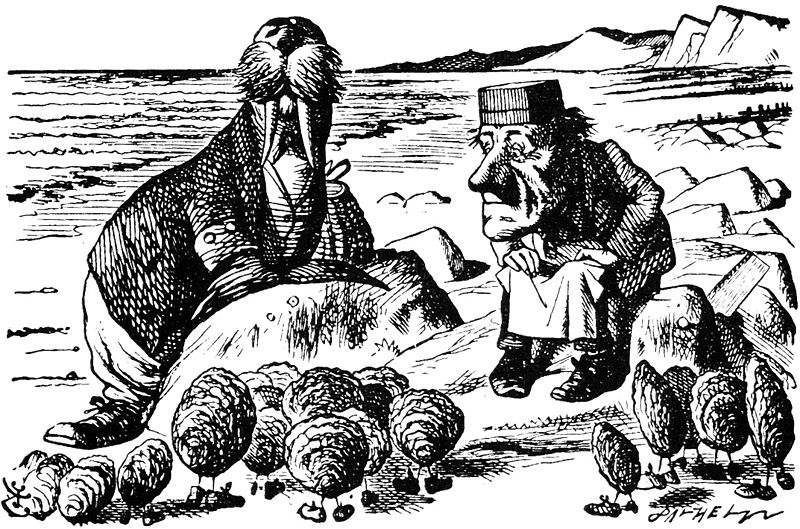
\includegraphics{800px-Briny_Beach.jpg}
% \end{center}
% \caption[Poem]{The Walrus and the Carpenter}
% \label{fig:walrus}
% \end{figure}

% \subsection{The Black Kitten}
%   One thing was certain, that the WHITE kitten had had nothing to
% do with it:---it was the black kitten's fault entirely~\cite{aiw}.  For the
% white kitten had been having its face washed by the old cat for
% the last quarter of an hour (and bearing it pretty well,
% considering); so you see that it COULDN'T have had any hand in
% the mischief.

%   The way Dinah washed her children's faces was this:  first she
% held the poor thing down by its ear with one paw, and then with
% the other paw she rubbed its face all over, the wrong way,
% beginning at the nose:  and just now, as I said, she was hard at
% work on the white kitten, which was lying quite still and trying
% to purr---no doubt feeling that it was all meant for its good.

%   But the black kitten had been finished with earlier in the
% afternoon, and so, while Alice was sitting curled up in a corner
% of the great arm-chair, half talking to herself and half asleep,
% the kitten had been having a grand game of romps with the ball of
% worsted Alice had been trying to wind up, and had been rolling it
% up and down till it had all come undone again; and there it was,
% spread over the hearth-rug, all knots and tangles, with the
% kitten running after its own tail in the middle.

% \subsection{The Reproach}

%   `Oh, you wicked little thing!' cried Alice, catching up the
% kitten, and giving it a little kiss to make it understand that it
% was in disgrace.  `Really, Dinah ought to have taught you better
% manners!  You OUGHT, Dinah, you know you ought!' she added,
% looking reproachfully at the old cat, and speaking in as cross a
% voice as she could manage---and then she scrambled back into the
% arm-chair, taking the kitten and the worsted with her, and began
% winding up the ball again.  But she didn't get on very fast, as
% she was talking all the time, sometimes to the kitten, and
% sometimes to herself.  Kitty sat very demurely on her knee,
% pretending to watch the progress of the winding, and now and then
% putting out one paw and gently touching the ball, as if it would
% be glad to help, if it might.

%   `Do you know what to-morrow is, Kitty?' Alice began.  `You'd
% have guessed if you'd been up in the window with me---only Dinah
% was making you tidy, so you couldn't.  I was watching the boys
% getting in stick for the bonfire---and it wants plenty of
% sticks, Kitty!  Only it got so cold, and it snowed so, they had
% to leave off.  Never mind, Kitty, we'll go and see the bonfire
% to-morrow.'  Here Alice wound two or three turns of the worsted
% round the kitten's neck, just to see how it would look:  this led
% to a scramble, in which the ball rolled down upon the floor, and
% yards and yards of it got unwound again.

%   `Do you know, I was so angry, Kitty,' Alice went on as soon as
% they were comfortably settled again, `when I saw all the mischief
% you had been doing, I was very nearly opening the window, and
% putting you out into the snow!  And you'd have deserved it, you
% little mischievous darling!  What have you got to say for
% yourself?  Now don't interrupt me!' she went on, holding up one
% finger.  `I'm going to tell you all your faults.  Number one:
% you squeaked twice while Dinah was washing your face this
% morning.  Now you can't deny it, Kitty:  I heard you!  What that
% you say?' (pretending that the kitten was speaking.)  `Her paw
% went into your eye?  Well, that's YOUR fault, for keeping your
% eyes open---if you'd shut them tight up, it wouldn't have
% happened.  Now don't make any more excuses, but listen!  Number
% two:  you pulled Snowdrop away by the tail just as I had put down
% the saucer of milk before her!  What, you were thirsty, were you?
